%\chapter{List of Definitions}
\chapter{Preliminaries}\label{chapter:list-of-definitions}

%The reader does not need to go through this chapter first of all. In the following chapters, we redirect the reader to this chapter to refer the definitions of certain graph classes or problems in NP. The reader can refer the same if required as we go step-by-step into the theory that we establish in this text. The reader can go through the complexity notations (\Cref{section:complexity-notation-functions}) and definition of symbols (\Cref{section:definitions-for-symbols}), otherwise the reader may omit this chapter (for now) and start going through from \Cref{chapter:introduction}.

\section{Complexity notation functions}\label{section:complexity-notation-functions}

The following functions \cite{Cormen} are used to denote the complexity \index{complexity notations} of algorithms in terms of the input size $n$. The exact runtime complexity of an algorithm is returned by $g(n)$, a function of $n$.\\

{\boldmath$\Theta$}

$\Theta(g(n)) = \{f(n) : \exists\ c_1>0, c_2>0$ and $n_0>0$ such that \[0 \leq c_1\ g(n) \leq f(n)\leq c_2\ g(n)\ \forall\ n\geq n_0\}
\]

{\boldmath$O$}

$O(g(n)) = \{f(n) : \exists\ c>0$ and $n_0>0$ such that \[0 \leq f(n)\leq c\ g(n)\ \forall\ n\geq n_0\}
\]

{\boldmath$\Omega$}

$\Omega(g(n)) = \{f(n) : \exists\ c>0$ and $n_0>0$ such that \[0 \leq c\ g(n) \leq f(n)\ \forall\ n>n_0\}
\]

{\boldmath$o$}

$o(g(n)) = \{f(n) : \forall\ c>0\ \exists\ n_0>0$ such that \[0 \leq f(n) < c\ g(n)\ \forall\ n\geq n_0\}
\]

{\boldmath$\omega$}

$\omega(g(n)) = \{f(n) : \forall\ c>0\ \exists\ n_0>0$ such that \[0 \leq c\ g(n) < f(n)\ \forall\ n\geq n_0\}
\]

\section{Definitions for symbols}\label{section:definitions-for-symbols}

Referring from the list of symbols.\\

\textbf{Left sequential union}\index{left sequential union}: If $P = (a,b)$, then after executing the statement $P = P \cup_{\setminus s} (c)$, $P$ becomes $(c, a, b)$. This operation can add a single element to a sequence, or merge two sequences.\\

\textbf{Right sequential union}\index{right sequential union}: If $P = (b,c)$, then after executing the statement $P = P \cup_{s/} (a)$, $P$ becomes $(b, c, a)$. This operation can add a single element to a sequence, or merge two sequences.\\

\textbf{Infimum}: The infimum of a subset $X$ of a set $X^\prime$ is the largest element of $X^\prime$ which is less than or equal to all the elements in $X$.\\

\textbf{Ceiling}: Let $x$ be a real number, then $i = \lceil x\rceil$ is the smallest integer such that $i \geq x$.\\

\textbf{Floor}: Let $x$ be a real number, then $i = \lfloor x\rfloor$ is the biggest integer such that $i \leq x$.\\

\textbf{Setminus}\index{setminus}: It removes the elements from the set preceding the operation symbol which are common to the set succeeding it. If $A = \{a, b, c\}$ and $B = \{b, c\}$ are two sets, then $A \setminus B = \{c\}$. For the sake of another example if $A = \{a, b, c\}$ and $B = \{c, d, e\}$ are two sets, then $A \setminus B = \{a, b\}$.\\

\textbf{Shortest distance between vertices}\index{shortest distance}: This statement returns the number of edges in a shortest path between two vertices $x$ and $y$.\\

\textbf{Adjacency at a distance {\boldmath$1$}}: This statement returns the set of vertices that are adjacent to $X$, excluding $X$. $X$ can be a single vertex, a set of vertices, or a subgraph of $G$.\\

\textbf{Adjacency at a distance {\boldmath$i$}}\index{adjacency}: This statement returns the set of vertices that are atmost at a distance $i$ from $X$, excluding $X$. $X$ can be a single vertex, a set of vertices, or a subgraph of $G$.\\

\textbf{Edge set in graph {\boldmath$G$}}\index{edge set in a graph}. This keyword acts as a variable which denotes the edge set in graph $G$.\\

\textbf{Neighbourhood at a distance {\boldmath$1$}}: This statement returns the set of vertices that are adjacent to $X$, including $X$. $X$ can be a single vertex, a set of vertices, or a subgraph of $G$.\\

\textbf{Neighbourhood at a distance {\boldmath$i$}}\index{neighbourhood}: This statement returns the set of vertices that are atmost at a distance $i$ from $X$, including $X$. $X$ can be a single vertex, a set of vertices, or a subgraph of $G$.\\

\textbf{Vertex set in graph {\boldmath$G$}}\index{vertex set in a graph}: This keyword acts as a variable which denotes the vertex set in graph $G$.\\

\textbf{Shortest path function}\index{shortest path}: A function that returns the shortest path $P$ from $u$ to $v$; the sequence of vertices in $P$ from $u$ to $v$, including $u$ and $v$.

\section{Problems in NP}\label{section:problems-in-NP}

The following problems are mentioned in the following chapters.\\

\textbf{\textit{Distinct 3-partition problem}}: In a \textit{distinct 3-partition problem} \index{distinct 3-partition problem}, given input is a set of positive integers, $X = \{a_1, a_2, . . ., a_{3n}\}$, and a positive integer $B$ such that $\sum_{i=1}^{3n}a_i = nB, \frac{B}{4}>a_i>\frac{B}{2}$; the task is to find if $X$ can be partitioned into $n$ sets, each containing $3$ integers, such that each set sums to $B$.\\

\textbf{\textit{Determination of a Hamiltonian cycle}}: A\textbf{\textit{Hamiltonian cycle}} \index{Hamiltonian cycle} of a graph $G$ is a path $P=(v_1,v_2,\dots,v_n,v_1)$ such that $n=|G.V|$ and for every pair of adjacent vertices $v_i$ and $v,j$ in $P$, $(v_i,v_j)\in G.E$. One approach to determine whether a hamiltonian cycle exists in a graph $G$ can be done as follows: we can check for every possible sequence of vertices $G.V$ that it satisfies the constraint or not. If there is at least one such sequence, the return value is $true$, otherwise $false$. This approach takes $O(n^n)$ time.\\

\textbf{\textit{Graph coloring problem}}\index{vertex coloring}: Given a graph $G$ and a set of infinite colors $C$, the task is to find the minimum number of colors in $C$ which can be assigned to each vertex in $G.V$, such that (1) each vertex is colored with only one color, and (2) $\forall\ a,b \in G.V$, if $(a,b) \in G.E$, then $color(a) \neq color(b)$. One solution is to color vertices sequentially, for each sequence of vertices in $G.V$. The sequence of vertices which utilizes the least amount of colors is the final solution. This approach takes $O(n^n)$ time.\\

\textbf{\textit{Graph isomorphism problem}}\index{isomorphism in graphs}: Given two graphs $G_1$ and $G_2$ such that $|G_1.V| = |G_2.V|$, the task is to determine if $\exists$ a sequence of vertices $C_1$ of $G_1.V$ and a sequence of vertices $C_2$ of $G_2.V$ such that $\forall\ 1\leq i,j\leq |G_1.V|: i\neq j$, $(C_2[i],C_2[j]) \in G_2.E$ if and only if $(C_1[i],C_1[j]) \in G_1.E$. One possible solution is to compare one sequence of $G_1.V$ with all the possible sequences of $G_2.V$. If the constraints get satisfies get satisfies at least once, then the value $true$ is returned, otherwise $false$. This approach takes $O(n^n)$ time.\\

\textbf{\textit{Knapsack problem}}: The input is a set of non-divisible objects have some associated weight and value, and a knapsack of a weight-capacity $k$. The objective is to fill the objects (repetition of one type to object is possible indefinitely) in the knapsack such that the total value is maximum.\\

\textbf{\textit{Largest Clique problem}}\index{largest clique problem}: Given a graph $G$, the task is to find the largest set of vertices $C\subseteq G.V$ such that $\forall\ a,b \in C$, if $a\neq b$ then $(a,b) \in G.E$. A possible solution is to check for each possible subset of $G.V$ that satisfy the constraint. The largest of all such sets is the solution. This approach takes $O(2^n)$ time.\\

\textbf{\textit{Maximum independent set problem}}\index{independent set maximum size}: Given a graph $G$, the task is to find the set of vertices $C\subseteq G.V$, of greatest possible size such that $\forall\ a,b \in G.V$, for all $(a,b) \in G.E$, if $a \in C$, then $b \not\in C$. A possible solution is to check for each possible subset of $G.V$ that satisfy the constraint. The largest of all such sets is the solution. This approach takes $O(2^n)$ time.\\

\textbf{\textit{Minimum vertex cover problem}}\index{minimum vertex cover problem}: Given a graph $G$, the task is to find the set of vertices $C\subseteq G.V$, of least possible size such that $\forall\ (a,b) \in G.E$, either $a \in C$ or $b\in C$ or both $a,b \in C$. A possible solution is to check for each possible subset of $G.V$ that satisfy the constraint. The smallest of all such sets is the solution. This approach takes $O(2^n)$ time.\\

\textbf{\textit{Minimum dominating set problem}}\index{minimum dominating set}: Given a graph $G$, the task is to compute a subset $D$ of $G.V$ of minimum size such that each vertex in $G.V\setminus D$ is connected to at least one vertex in $D$ by an edge.\\

\textbf{\textit{Rod cutting problem}}: Given is the length of a rod $L$ and a list of profit $p_i$ corresponding to all the possible lengths $i$ of the rod $C = \{p_i, i\}_{i=1}^L: i\in\mathbb{N}$. The task is to find how the rod should be cut in order to maximize the profit. One solution is to assume that the rod of length $L$ units can be cut at $L-1$ positions. Then compute the cost of each cut-decisions' sequence. The sequence which produces the maximum of the costs is the output. This procedure takes $O(2^{L-1})$ time.

\section{Graph Classes}

The following are a few graph classes with their definitions.

\subsection{Spider graphs}

\index{spider graphs}In a \textit{spider graph} (as per the usage in this text), only one vertex $c$, the head vertex, is of degree $d \geq 3$; the degree of all other vertices is less than $3$, it is either $2$ or $1$. An example spider graph is presented in \Cref{figure:example-spider-graph}. {\boldmath$SP(s,r)$} \index{$SP(s,r)$} is a spider graph with degree $s$ of head $c$, and length of each arm $r$.

\begin{figure}
    \centering
    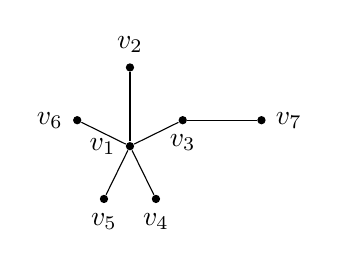
\begin{tikzpicture}
        \node [circle, fill=black, inner sep=0pt, minimum size=3pt, label=left:{$v_1$}] (A) at (0,0) {};
        \node [circle, fill=black, inner sep=0pt, minimum size=3pt, label=above:{$v_2$}] (B) at (0,1) {};
        \node [circle, fill=black, inner sep=0pt, minimum size=3pt, label=below:{$v_3$}] (C) at (.67,.33) {};
        \node [circle, fill=black, inner sep=0pt, minimum size=3pt, label=below:{$v_4$}] (D) at (.33,-.67) {};
        \node [circle, fill=black, inner sep=0pt, minimum size=3pt, label=below:{$v_5$}] (E) at (-.33,-.67) {};
        \node [circle, fill=black, inner sep=0pt, minimum size=3pt, label=left:{$v_6$}] (F) at (-.67,.33) {};
        \node [circle, fill=black, inner sep=0pt, minimum size=3pt, label=right:{$v_7$}] (G) at (1.67,.33) {};
        
        \draw (A) -- (B); \draw (A) -- (C); \draw (A) -- (D); \draw (A) -- (E); \draw (A) -- (F);
        \draw (C) -- (G);
    \end{tikzpicture}
    \caption{An example spider graph.}
    \label{figure:example-spider-graph}
\end{figure}

\subsection{\texorpdfstring{\boldmath$P_k$}{p-k}-free graphs}

{\boldmath$P_k$} \index{$P_k$} is a path of $k$ vertices ($k-1$ edges). A graph $G$ is $P_k-free$ \index{$P_k$-free graphs} if any induced subgraph of $G$ does not contain $P_k$.

\subsection{Cographs}\label{subsection:cographs}

\textit{Cographs} \index{cographs} can be recursively defined as follows. A single vertex is a cograph. A disjoint union of two cographs is a cograph. A complete join of two cographs is a cograph. Graph complement of a cograph is a cograph, which is why, cographs are also called \textbf{\textit{complement-reducible graphs}}\index{complement-reducible graphs}. Cographs are $P_4$-free graphs. A few examples of (recursively) constructed cographs are presented in \Cref{figure:example-cographs}.

\begin{figure}
    \centering
    \subfigure[]{
        \begin{tikzpicture}
            \node [circle, fill=black, inner sep=0pt, minimum size=3pt, label=below:{$v$}] at (0,0) {};
        \end{tikzpicture}
    }
    \subfigure[]{
        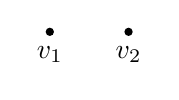
\begin{tikzpicture}
            \node [circle, fill=black, inner sep=0pt, minimum size=3pt, label=below:{$v_1$}] at (0,0) {};
            \node [circle, fill=black, inner sep=0pt, minimum size=3pt, label=below:{$v_2$}] at (1,0) {};
        \end{tikzpicture}
    }
    \subfigure[]{
        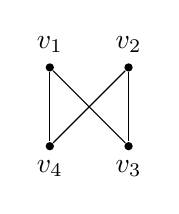
\begin{tikzpicture}
            \node [circle, fill=black, inner sep=0pt, minimum size=3pt, label=above:{$v_1$}] (A) at (0,0) {};
            \node [circle, fill=black, inner sep=0pt, minimum size=3pt, label=above:{$v_2$}] (B) at (1,0) {};
            
            \node [circle, fill=black, inner sep=0pt, minimum size=3pt, label=below:{$v_3$}] (C) at (1,-1) {};
            \node [circle, fill=black, inner sep=0pt, minimum size=3pt, label=below:{$v_4$}] (D) at (0,-1) {};
            
            \draw (A) -- (C); \draw (A) -- (D);
            \draw (B) -- (C); \draw (B) -- (D);
        \end{tikzpicture}
    }
    \subfigure[]{
        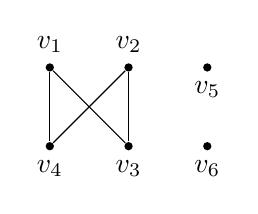
\begin{tikzpicture}
            \node [circle, fill=black, inner sep=0pt, minimum size=3pt, label=above:{$v_1$}] (A) at (0,0) {};
            \node [circle, fill=black, inner sep=0pt, minimum size=3pt, label=above:{$v_2$}] (B) at (1,0) {};
            
            \node [circle, fill=black, inner sep=0pt, minimum size=3pt, label=below:{$v_3$}] (C) at (1,-1) {};
            \node [circle, fill=black, inner sep=0pt, minimum size=3pt, label=below:{$v_4$}] (D) at (0,-1) {};
            
            \node [circle, fill=black, inner sep=0pt, minimum size=3pt, label=below:{$v_5$}] (E) at (2,0) {};
            \node [circle, fill=black, inner sep=0pt, minimum size=3pt, label=below:{$v_6$}] (F) at (2,-1) {};
            
            \draw (A) -- (C); \draw (A) -- (D);
            \draw (B) -- (C); \draw (B) -- (D);
        \end{tikzpicture}
    }
    \subfigure[]{
        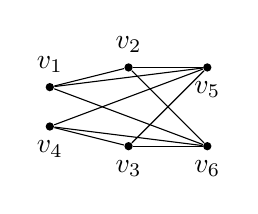
\begin{tikzpicture}
            \node [circle, fill=black, inner sep=0pt, minimum size=3pt, label=above:{$v_1$}] (A) at (0,-.25) {};
            \node [circle, fill=black, inner sep=0pt, minimum size=3pt, label=above:{$v_2$}] (B) at (1,0) {};
            
            \node [circle, fill=black, inner sep=0pt, minimum size=3pt, label=below:{$v_3$}] (C) at (1,-1) {};
            \node [circle, fill=black, inner sep=0pt, minimum size=3pt, label=below:{$v_4$}] (D) at (0,-.75) {};
            
            \node [circle, fill=black, inner sep=0pt, minimum size=3pt, label=below:{$v_5$}] (E) at (2,0) {};
            \node [circle, fill=black, inner sep=0pt, minimum size=3pt, label=below:{$v_6$}] (F) at (2,-1) {};
            
            \draw (A) -- (B);
            \draw (A) -- (E); \draw (A) -- (F);
            \draw (B) -- (E); \draw (B) -- (F);
            
            \draw (C) -- (D);
            \draw (C) -- (E); \draw (C) -- (F);
            \draw (D) -- (E); \draw (D) -- (F);
        \end{tikzpicture}
    }
    \caption{a: a single vertex is a \textit{cograph}; b: a disjoint union of two copies of the \textit{cograph} in (a) is a \textit{cograph}; c: a complete join of two copies of the \textit{cograph} in (b) is a cograph; d: a disjoint union of the \textit{cographs} in (b) and (c) is a \textit{cograph}; e: the graph complement of the \textit{cograph} in (d) is a \textit{cograph}.}
    \label{figure:example-cographs}
\end{figure}

\subsubsection{Reviewing cograph theory}

A cotree \cite{Corneil1981}, constructed from a cograph, assists in the computation of properties of a cograph in linear time, such as \textit{maximum independent set}, \textit{graph coloring number}, and determining if there exists a Hamiltonian cycle. A cograph can be recognized in linear time, and cotrees can be constructed using modular decomposition \cite{Corneil1985}, partition refinement \cite{Habib2005}, LexBFS \cite{Bretscher2008}, or split decomposition \cite{Gioan2012}.  An induced subgraph of a cograph is a cograph itself \cite{Damaschke1990}.

\subsection{Disk Graphs}

A graph $G$ is a \textit{disk graph} \index{disk graphs} if there is an edge between a pair of vertices iff the circles drawn on the plane with those vertices as centers overlap. These circles can generally be of arbitrary radius. If radius of all the circles overlap, the graph is called a \textbf{\textit{unit disk graph}}.

For example, let a circle $C$ of radius $R=2$ be positioned on the plane at $(0,0)$, three more disks $c_1$, $c_2$ and $c_3$, each of radius $r=1$, is placed with their centres respectively at $(2,0)$, $(0,2)$, and $(-2,0)$. Let us assume that a chain of $4$ disks $Ch_1=(c_1^1, c_1^2, c_1^3, c_1^4)$ is attached to $c_1$ such that $c_1^1$ overlaps with $c_1$ and $c_1^2$ only, $c_1^4$ overlaps with $c_1^3$ only, and $\forall\ 2 \leq j \leq 3$, $c_1^j$ overlap with only $c_1^{j-1}$ and $c_1^{j+1}$. Exactly in the similar way, there is a chain behind each of $c_2$ ($Ch_2=(c_2^1, c_2^2, c_2^3, c_2^4)$) and $c_3$ ($Ch_3=(c_3^1, c_3^2, c_3^3, c_3^4)$).

There are $q=3$ chains of disks, and $p=4$ more disks behind the first disk in each chain. Let $Ch = \{Ch_1, Ch_2, Ch_3\}$ and $Cir = \{c_1, c_2, c_3\}$ We denote this network of disks by $DK(R$, $r$, $q$, $p$, $C$, $Cir$, $Ch) = DK(2$, $1$, $3$, $4$, $C$, $Cir$, $Ch)$.

Let the vertex corresponding to $C$ be called head $h$, vertices corresponding to $c_i$ be called $v_i$, and the vertices corresponding to $c_i^j$ be called $v_i^j$, $\forall\ 1 \leq i \leq 3$, and $\forall\ 1 \leq j \leq 4$. The graph formed by this setting will be a spider graph $SP(3,5)$, as shown in \Cref{figure:example-disk-graph-1}.

%\newcounter{c}
\begin{figure}
    \centering
    \subfigure[]{
        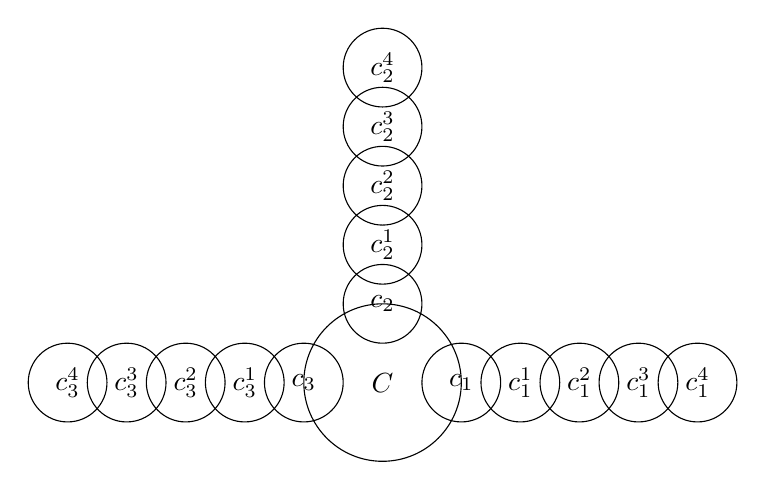
\begin{tikzpicture}[scale=0.5]
            \draw (0,0) circle (2); \node at (0,0) {$C$};
                
            \draw (2,0) circle (1); \node at (2,0) {$c_1$};
            \draw (3.5,0) circle (1); \node at (3.5,0) {$c_1^1$};
            \draw (5,0) circle (1); \node at (5,0) {$c_1^2$};
            \draw (6.5,0) circle (1); \node at (6.5,0) {$c_1^3$};
            \draw (8,0) circle (1); \node at (8,0) {$c_1^4$};
            
            \draw (0,2) circle (1); \node at (0,2) {$c_2$};
            \draw (0,3.5) circle (1); \node at (0,3.5) {$c_2^1$};
            \draw (0,5) circle (1); \node at (0,5) {$c_2^2$};
            \draw (0,6.5) circle (1); \node at (0,6.5) {$c_2^3$};
            \draw (0,8) circle (1); \node at (0,8) {$c_2^4$};
            
            \draw (-2,0) circle (1); \node at (-2,0) {$c_3$};
            \draw (-3.5,0) circle (1); \node at (-3.5,0) {$c_3^1$};
            \draw (-5,0) circle (1); \node at (-5,0) {$c_3^2$};
            \draw (-6.5,0) circle (1); \node at (-6.5,0) {$c_3^3$};
            \draw (-8,0) circle (1); \node at (-8,0) {$c_3^4$};
        \end{tikzpicture}
    }
    \subfigure[]{
        \begin{tikzpicture}
            \node [circle, fill=black, inner sep=0pt, minimum size=3pt, label=above:{$h$}] (C) at (0,0) {};
            
            \node [circle, fill=black, inner sep=0pt, minimum size=3pt, label=above:{$v_1$}] (A) at (1,1) {};
            \node [circle, fill=black, inner sep=0pt, minimum size=3pt, label=above:{$v_2$}] (B) at (1,0) {};
            \node [circle, fill=black, inner sep=0pt, minimum size=3pt, label=above:{$v_3$}] (D) at (1,-1) {};
            
            \draw (A) -- (C); \draw (B) -- (C); \draw (D) -- (C);
                
            \setcounter{c}{1}
            \loop
                \node [circle, fill=black, inner sep=0pt, minimum size=3pt, label=above:{$v_1^{\thec}$}] (AA) at (\value{c}+1,1) {};
                \node [circle, fill=black, inner sep=0pt, minimum size=3pt, label=above:{$v_2^{\thec}$}] (AB) at (\value{c}+1,0) {};
                \node [circle, fill=black, inner sep=0pt, minimum size=3pt, label=above:{$v_3^{\thec}$}] (AD) at (\value{c}+1,-1) {};
                
                \stepcounter{c}
                \ifnum \value{c} < 5
                    \repeat
                    
            \draw (AA) -- (A); \draw (AB) -- (B); \draw (AD) -- (D);
            
        \end{tikzpicture}
    }
    \caption{(a) arrangement of disks and (b) the corresponding disk graph, geometrically not according to the arrangement of the disks, but connections according to the overlap of respective disks.}
    \label{figure:example-disk-graph-1}
\end{figure}

Another example of an arrangement of disks is shown in \Cref{figure:example-disk-graph-2}.

\begin{figure}
    \centering
    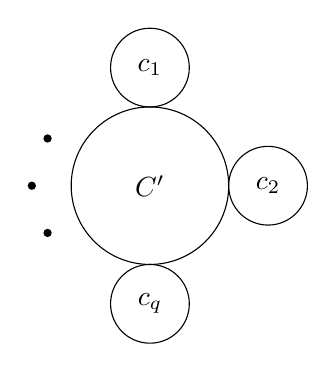
\begin{tikzpicture}
        \draw (0,0) circle (1); \node at (0,0) {$C^\prime$};
        
        \draw (0,1.5) circle (.5); \node at (0,1.5) {$c_1$};
        \draw (1.5,0) circle (.5); \node at (1.5,0) {$c_2$};
        \node [circle, fill=black, inner sep=0pt, minimum size=3pt] (D) at (-1.5+.2,.6) {};
        \node [circle, fill=black, inner sep=0pt, minimum size=3pt] (D) at (-1.5,0) {};
        \node [circle, fill=black, inner sep=0pt, minimum size=3pt] (D) at (-1.5+.2,-.6) {};
        \draw (0,-1.5) circle (.5); \node at (0,-1.5) {$c_q$};
    \end{tikzpicture}
    \caption{Central disk {$C^\prime$} and a set of $Cir = \{c_1, c_2, ..., c_q\}$ disks with their circumference touching the circumference of {$C^\prime$}, and not overlaping with each other, or with $C^\prime$}
    \label{figure:example-disk-graph-2}
\end{figure}

\subsubsection{Reviewing disk graph theory}

Computation of various properties on disk graph is NP-Hard. Clark et al. (1990) \cite{Clark1990} showed that finding the chromatic number of disk graph is NP-Complete. They also showed that 3-coloring problem is NP-Complete on unit disk graph, even if their underlying disk representation is given. Although, in contrast, they also gave a polynomial time algorithm to find maximal cliques in unit disk graph when the geometrical representation of the underlying disks is given.

\subsection{Interval Graphs}\label{subsection:interval-graphs}

An \textit{interval graph} \index{interval graphs} is formed from a set of intervals on the real line where each interval is represented as a vertex and there is an edge between two vertices if an only if their corresponding intervals overlap on the real line.

\subsubsection{Interval graphs from a set of intervals}

The input is the list of intervals $L$, each interval $i$ has a starting time $s_i$ and an ending time $e_i$. Each interval in $L$ corresponds to a vertex in $G$.

To convert a set of intervals to an interval graph, for each interval $a$ $\in$ $L$, a vertex $v_a$ is added to $G$.$V$. Wherever there is an overlap between any two distinct intervals $a$ and $b$, $a$, $b$ $\in$ $L$, that is, if $s_b$ $\geq$ $s_a$ and $s_b < e_a$, we add an edge ($v_a$, $v_b$) in $G.E$. After following this procedure, $G$ represents the interval graph corresponding to $L$. This is demonstrated in \Cref{figure:example-interval-graph}.

\begin{figure}
    \centering
    \subfigure[]{
		\begin{tikzpicture}
			\draw (-4, 0) -- (-3, 0);
			\draw (-4, 0.5) -- (-3, 0.5);
			\draw (-3.5, 1) -- (-1.5, 1);
			\draw (-3.25, -0.5) -- (0.25, -0.5);
			\draw (-2, 0) -- (-1, 0);
			
			\draw (0, 0) -- (1, 0);
			\draw (0.75, 0.5) -- (2.5, 0.5);
			\draw (2, 0) -- (3, 0);
			\draw (2, -0.5) -- (3, -0.5);
			
			\node at (-3.5, 0.75) {$1$};
			\node at (-3.5, 0.25) {$2$};
			\node at (-2.5, 1.25) {$3$};
			\node at (-1.75, -0.25) {$4$};
			\node at (-1.5, 0.25) {$5$};
			
			\node at (0.5, 0.25) {$6$};
			\node at (1.625, 0.75) {$7$};
			\node at (2.5, 0.25) {$8$};
			\node at (2.5, -0.25) {$9$};
		\end{tikzpicture}
	}
	\subfigure[]{
		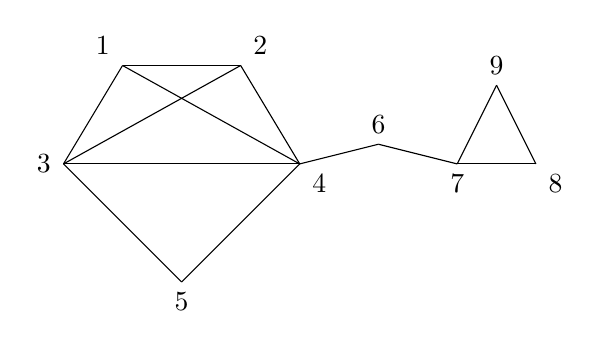
\begin{tikzpicture}
			\draw (-4, 0) -- (-1, 0);
			
			\draw (-3.25, 1.25) -- (-1.75, 1.25);
			\draw (-4, 0) -- (-3.25, 1.25);
			\draw (-1.75, 1.25) -- (-1, 0);
			\draw (-4, 0) -- (-1.75, 1.25);
			\draw (-3.25, 1.25) -- (-1, 0);
			
			\draw (-4, 0) -- (-2.5, -1.5);
			\draw (-2.5, -1.5) -- (-1, 0);
			
			\draw (-1, 0) -- (0, 0.25);
			
			\draw (0, 0.25) -- (1, 0);
			
			\draw (1, 0) -- (2, 0);
			
			\draw (1, 0) -- (1.5, 1);
			\draw (1.5, 1) -- (2, 0);
			
			\node at (-3.5, 1.5) {$1$};
			\node at (-1.5, 1.5) {$2$};
			\node at (-4.25, 0) {$3$};
			\node at (-0.75, -0.25) {$4$};
			\node at (-2.5, -1.75) {$5$};
			
			\node at (0, 0.5) {$6$};
			\node at (1, -0.25) {$7$};
			\node at (2.25, -0.25) {$8$};
			\node at (1.5, 1.25) {$9$};
		\end{tikzpicture}
	}
	\caption{An example set of intervals (a) and the corresponding interval graph (b).}
	\label{figure:example-interval-graph}
\end{figure}

As demonstrated in \Cref{figure:example-interval-graph-frames}, we can also imagine this procedure as follows. We imagine that a vertical line that traverses the intervals from left to right (we could otherwise do right to left). The vertical line will intersect the horizontal intervals while traversal, it may intersect zero, one, or more intervals at a particular instant. We draw a clique between the corresponding vertices for each distinct set of intervals that the vertical line intersects. Each distinct instance that can possibly be presented by the position of the vertical line is called a \textit{frame}.

\begin{figure}
	\centering
	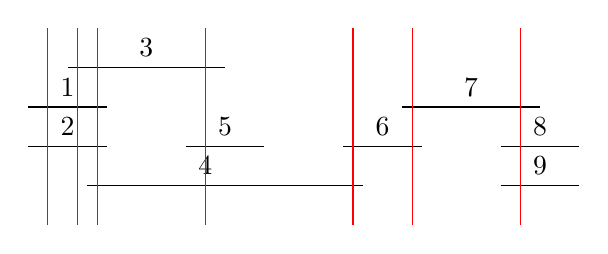
\begin{tikzpicture}
		\draw (-4, 0) -- (-3, 0);
		\draw (-4, 0.5) -- (-3, 0.5);
		\draw (-3.5, 1) -- (-1.5, 1);
		\draw (-3.25, -0.5) -- (0.25, -0.5);
		\draw (-2, 0) -- (-1, 0);
		
		\draw (0, 0) -- (1, 0);
		\draw (0.75, 0.5) -- (2.5, 0.5);
		\draw (2, 0) -- (3, 0);
		\draw (2, -0.5) -- (3, -0.5);
		
		\node at (-3.5, 0.75) {$1$};
		\node at (-3.5, 0.25) {$2$};
		\node at (-2.5, 1.25) {$3$};
		\node at (-1.75, -0.25) {$4$};
		\node at (-1.5, 0.25) {$5$};
		
		\node at (0.5, 0.25) {$6$};
		\node at (1.625, 0.75) {$7$};
		\node at (2.5, 0.25) {$8$};
		\node at (2.5, -0.25) {$9$};
		
		\draw[red] (-3.75, 1.5) -- (-3.75, -1);
		\draw[red] (-3.375, 1.5) -- (-3.375, -1);
		\draw[red] (-3.125, 1.5) -- (-3.125, -1);
		\draw[red] (-1.75, 1.5) -- (-1.75, -1);
		\draw[red] (0.125, 1.5) -- (0.125, -1);
		\draw[red] (0.875, 1.5) -- (0.875, -1);
		\draw[red] (2.25, 1.5) -- (2.25, -1);
	\end{tikzpicture}
	\caption{Positions of the vertical line while traversing an example set on intervals on the real line. This figure presents each frame where a new untraversed interval is encountered and a clique in the graph (in \Cref{figure:example-interval-graph}-(b)) is added.}
	\label{figure:example-interval-graph-frames}
\end{figure}

\subsection{Similarity between a path and an interval graph}\label{subsection:IG-path-similar}

\begin{proposition}\label{proposition:LongestPathLIG}
Let $l,r\in L$ be two intervals such that $P_L$ (shortest path between $l$ and $r$) is of maximum length as compared to shortest path between any pair of intervals in $L$. Then, for each interval $i\in L$, if $i\not\in P_L$, then $i$ shall overlap with at least one interval of $P_L$.
\end{proposition}

\begin{proof}
Let $s = \min s_j:j\in P_L$ and $e = \max e_j:j\in P_L$. Let that $i$ does not overlap with any interval in $L$, then either (1) $e_i < s$, or (2) $s_i > e$.

First let $e_i < s$ for contradiction. Let $P_L^\prime$ be the shortest path between $i$ and $l$, and $P_L^{\prime\prime}$ be the shortest path between $i$ and $r$. Here, we obtain a contradiction because $P_L^{\prime\prime} \geq P_L + P_L^\prime-1$ and $P^\prime \geq 2$ $|P_L^{\prime\prime}|$, so $P_L$ is not of maximum length. Otherwise, $L$ may be disconnected.

Similarly, we can obtain a contradiction for an interval $i$ such that $s_i > e_r$.
\end{proof}

\begin{corollary}\label{corollary:NHClosurePIG}
Let $P$ be the shortest path between a pair of vertices in $G$, which is of maximum length as compared to the shortest path between any other pair of vertices in $G.V$, that is, $P$ is the diameter of $G$, then all vertices in $G\setminus P$ are connected by a single edge with at least one of the vertices in $P$.
\end{corollary}

\Cref{corollary:NHClosurePIG} has been proved earlier in \cite{Kare2019} and \cite{Kamali2019,Kamali2020}. It can also be observed that the interval graphs do not contain a cycle of size more than $3$ \cite{Gilmore1964,Golumbic2004}; we show this in \Cref{proposition:IG-no-cycle}.

\begin{proposition}\label{proposition:IG-no-cycle}
For any induced subgraph $G^\prime$ of an interval graph $G$ with $|G^\prime.V| \neq 3,\ G^\prime$ will not be a cycle.
\end{proposition}

\begin{proof}
Let the interval graph be a cycle of $k \geq 4$ vertices $v_1$, $v_2$, $v_3$, $...$, $v_k$ corresponding to the intervals $i_1, i_2, i_3, ..., i_k$ respectively. The interval $i_j$ overlaps with interval $i_{j+1},\ \forall 1\leq j\leq k-1$. Now to validate this cycle, interval $i_1$ must overlap with $i_k$. This is only possible if either or both of the following occur.

(a) $i_1$ overlaps with all intervals $i_2, i_3, i_4, ..., i_{k-1}$ also.

(b) $i_k$ overlaps with all intervals $i_2, i_3, i_4, ..., i_{k-1}$ also.\\
Here we obtain the contradiction that there will not exist cycle of length greater than $3$ in any induced subgraph of $G$. This is demonstrated in \Cref{figure:IG-no-cycle}.
\end{proof}

\begin{figure}
	\centering
	\subfigure[]{
		\begin{tikzpicture}
			\draw (0, 0) -- (1, 0); \draw[dashed] (1, 0) -- (3.75, 0);
			\draw (0.75, -1) -- (1.75, -1);
			\draw (2.5, -3) -- (3.5, -3);
			\draw (3.25, -4) -- (4.25, -4);  \draw[dashed] (3.25, -4) -- (0.5, -4);
			
			\node at (0.5, -0.5) {$i_1$};
			\node at (1.3, -1.5) {$i_2$};
			
			\node [circle, fill=black, inner sep=0pt, minimum size=3pt] at (2,-1.75) {};
			\node [circle, fill=black, inner sep=0pt, minimum size=3pt] at (2.125,-2) {};
			\node [circle, fill=black, inner sep=0pt, minimum size=3pt] at (2.25,-2.25) {};
			
			\node at (3, -3.5) {$i_{k-1}$};
			\node at (3.8, -4.5) {$i_k$};
			
			\node at (2, -5) {\textit{Set of intervals}};
		\end{tikzpicture}
	}
	\subfigure[]{
		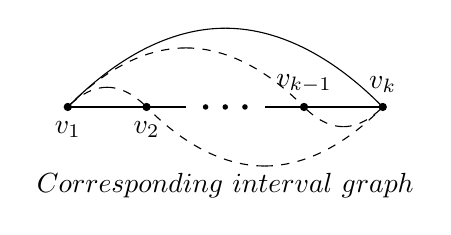
\begin{tikzpicture}
		    \node [circle, fill=black, inner sep=0pt, minimum size=3pt, label=below:{$v_1$}] at (0,0) {};
		    \node [circle, fill=black, inner sep=0pt, minimum size=3pt, label=below:{$v_2$}] at (1,0) {};
		    
		    \node [circle, fill=black, inner sep=0pt, minimum size=2pt] at (1.75,0) {};
		    \node [circle, fill=black, inner sep=0pt, minimum size=2pt] at (2,0) {};
		    \node [circle, fill=black, inner sep=0pt, minimum size=2pt] at (2.25,0) {};
		    
		    \node [circle, fill=black, inner sep=0pt, minimum size=3pt, label=above:{$v_{k-1}$}] at (3,0) {};
		    \node [circle, fill=black, inner sep=0pt, minimum size=3pt, label=above:{$v_k$}] at (4,0) {};
		    
			\draw (0,0) -- (1.5,0);
			\draw (4,0) -- (2.5,0);
			
			\draw (2,1) parabola (0,0); \draw (2,1) parabola (4,0);
			\draw[dashed] (1.5,.75) parabola (0,0); \draw[dashed] (1.5,.75) parabola (3,0);
			\draw[dashed] (.5,.25) parabola (0,0); \draw[dashed] (.5,.25) parabola (1,0);
			
			\draw[dashed] (2.5,-.75) parabola (4,0); \draw[dashed] (2.5,-.75) parabola (1,0);
			\draw[dashed] (3.5,-.25) parabola (4,0); \draw[dashed] (3.5,-.25) parabola (3,0);
			
			\node at (2,-1) {$Corresponding\ interval\ graph$};
		\end{tikzpicture}
	}
	\caption{Demonstration of what happens if we try to create an interval graph cycle and the corresponding set of intervals. The dotted lines are the prospective edges which shall form, apart from the original cycle of $k$ vertices. Either or both of the terminal vertices $v_1$ or $v_k$, on the original path $v_1, ..., v_k$ shall be connected to all the vertices from $v_2,v_3,\dots,v_{k-1}$.}
	\label{figure:IG-no-cycle}
\end{figure}

\begin{corollary}
We can conclude two simple facts, which are as follows.

(1) If a vertex $v$ of $G$ is not in $P$, then it is adjacent to some vertex in $P$, it is part of a clique involving that vertex of $P$.

(2) Each clique involves exactly

\quad (a) one vertex from $P$ or

\quad (b) two vertices from $P$ which are adjacent according to the sequence of $P$.
\end{corollary}

\subsubsection{Reviewing interval graph theory}

There are several linear time algorithms available to solve different problems on interval graph. Olariu \cite{Olariu1991} discovered linear time algorithm for coloring.  Marathe et al. \cite{Marathe1992} gave a linear time algorithm to compute minimum vertex cover. Similarly, a linear time algorithm to compute interval graph isomosphism was given in \cite{Lueker1979}. Ibarra \cite{Ibarra2017} proposed a linear time algorithm to compute the clique separator graph of a given interval graph. Fomin et al. \cite{Fomin2016} described an algorithm which solves the firefighter problem on interval graphs in $O(n^7)$ time. Interval graph ordering was introduced in \cite{Ramalingam1988}. As per interval graph ordering, the vertices are ordered according to the increasing order of the ending time of their corresponding intervals. Ravi et al. \cite{Ravi1992} proposed an algorithm to solve all pairs shortest path in $(O(n^2))$ time, where $n$ is the number of vertices. Authors in \cite{Kamali2019,Kamali2020}, along with \cite{Kare2019} discussed bounds on the burning number of interval graph. Although they have not provided any algorithm to find an optimal burning sequence.

\subsection{Permutation graphs}

A \textit{permutation graph} \index{permutation graphs} $G$ is constructed from an original sequence of numbers $O = (1, 2, 3, . . ., k)$ and its permutation $P = (p_1, p_2, p_3, . . ., p_k)$ such that there is an edge between vertices $v_i$ and $v_j$, corresponding to the numbers $i$ and $j$ in $O$, if $i < j$ in $O$, but $j$ occurs before $i$ in $P$. For example, let $O = (1, 2, 3, 4, 5, 6, 7, 8)$ and $P = (3, 1, 5, 2, 7, 4, 8, 6)$ be the subject permutation of $O$. Then the permutation graph $G$ formed from this pair $(O, P)$ is shown as \Cref{figure:example-permutation-graph}.

\begin{figure}
	\centering
	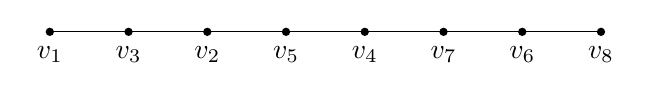
\begin{tikzpicture}
	    \draw (0,0) -- (7,0);
	    
	    \node [circle, fill=black, inner sep=0pt, minimum size=3pt, label=below:{$v_1$}] at (0,0) {};
		\node [circle, fill=black, inner sep=0pt, minimum size=3pt, label=below:{$v_3$}] at (1,0) {};
	    \node [circle, fill=black, inner sep=0pt, minimum size=3pt, label=below:{$v_2$}] at (2,0) {};
		\node [circle, fill=black, inner sep=0pt, minimum size=3pt, label=below:{$v_5$}] at (3,0) {};
	    \node [circle, fill=black, inner sep=0pt, minimum size=3pt, label=below:{$v_4$}] at (4,0) {};
	    \node [circle, fill=black, inner sep=0pt, minimum size=3pt, label=below:{$v_7$}] at (5,0) {};
	    \node [circle, fill=black, inner sep=0pt, minimum size=3pt, label=below:{$v_6$}] at (6,0) {};
		\node [circle, fill=black, inner sep=0pt, minimum size=3pt, label=below:{$v_8$}] at (7,0) {};
	\end{tikzpicture}
	\caption{Representation of permutation graph corresponding to $(O, P)$, where $O = (1, 2, 3, 4, 5, 6, 7, 8)$ and $P = (3, 1, 5, 2, 7, 4, 8, 6)$.}
	\label{figure:example-permutation-graph}
\end{figure}

\subsubsection{Reviewing permutation graph theory}

Polynomial time algorithms exist for various properties in permutation graphs. If $r$ is the size of longest decreasing subsequence in a permutation $P$, then the chromatic number and the size of largest clique in the corresponding permutation graph $G$, both are equal to $r$ \cite{Golumbic2004}.  Atallah et al. (1998) \cite{Atallah1988} proposed an algorithm that finds the minimum dominating set in an arbitrary permutation graph with $n$ vertices in $O(n\ \log^2 n)$ time.

\subsection{Split graphs}\label{subsection:split-graphs}

\index{split graphs}A graph $G$ is a \textit{split graph} if its vertices can be partitioned into a clique and an independent set. A split graph is $P_5$ free. An example split graph is presented in \Cref{figure:example-split-graph}

\begin{figure}
    \centering
    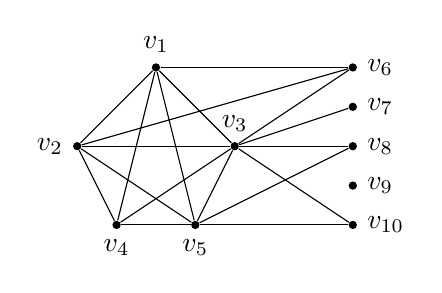
\begin{tikzpicture}
        \node [circle, fill=black, inner sep=0pt, minimum size=3pt, label=above:{$v_1$}] (A) at (0,0) {};
        \node [circle, fill=black, inner sep=0pt, minimum size=3pt, label=left:{$v_2$}] (B) at (-1,-1) {};
        \node [circle, fill=black, inner sep=0pt, minimum size=3pt, label=above:{$v_3$}] (C) at (1,-1) {};
        \node [circle, fill=black, inner sep=0pt, minimum size=3pt, label=below:{$v_4$}] (D) at (-.5,-2) {};
        \node [circle, fill=black, inner sep=0pt, minimum size=3pt, label=below:{$v_5$}] (E) at (.5,-2) {};
        
        \draw (A) -- (B); \draw (A) -- (C); \draw (A) -- (D); \draw (A) -- (E);
        \draw (B) -- (C); \draw (B) -- (D); \draw (B) -- (E);
        \draw (C) -- (D); \draw (C) -- (E);
        \draw (D) -- (E);
        
        \node [circle, fill=black, inner sep=0pt, minimum size=3pt, label=right:{$v_6$}] (F) at (2.5,0) {};
        \node [circle, fill=black, inner sep=0pt, minimum size=3pt, label=right:{$v_7$}] (G) at (2.5,-.5) {};
        \node [circle, fill=black, inner sep=0pt, minimum size=3pt, label=right:{$v_8$}] (H) at (2.5,-1) {};
        \node [circle, fill=black, inner sep=0pt, minimum size=3pt, label=right:{$v_9$}] (I) at (2.5,-1.5) {};
        \node [circle, fill=black, inner sep=0pt, minimum size=3pt, label=right:{$v_{10}$}] (J) at (2.5,-2) {};
        
        \draw (A) -- (F); \draw (B) -- (F); \draw (C) -- (F);
        \draw (C) -- (G);
        \draw (C) -- (H); \draw (E) -- (H);
        \draw (C) -- (J); \draw (E) -- (J);
    \end{tikzpicture}
    \caption{An example split graph. $C=\{v_1,v_2,\dots,v_5\}$ is the clique and $I=\{v_6,v_7,\dots,v_{10}\}$ is the independent set excerpt of this split graph.}
    \label{figure:example-split-graph}
\end{figure}

\subsubsection{Reviewing split graph theory}

Clearly, it is easy to compute the maximum clique on split graphs, and complementarily, its maximum independent set \cite{Golumbic2004,Hammer1981}; along with coloring. \cite{Kare2019} showed that split graphs can be burned in polynomial time. Determining if a hamiltonian cycle exists remains NP-Complete for split graphs\cite{Mueller1996}, along with the minimum dominating set problem \cite{Bertossi1984}.

% \bibliography{ref.bib}
% \bibliographystyle{plain}